\chapter{Rendering Surface Geometries using the NMM approach}
\label{chap:diffflssnmm}

In section $\ref{sec:snakegeomrenderings}$ we mentioned that we use the FLSS approach instead of the NMM apporach for producing our renderings applied on a snake mesh. The reason for choosing the FLSS approach was that it produces realiable results (according to its evaluation plots discussed in section $\ref{sec:virtualtestbench}$). Furthmore, the renderings resulting from the NMM approach look purplish compared to those produced by the FLSS approach as shown in figure $\ref{fig:appendixflssvsnmm}$. This figure shows renderings of our snake mesh when using an Elaphe grating produced by the FLSS approach (figure $\ref{fig:appendixcompflsselaphe}$) and the NMM approach (figure $\ref{fig:appendixcompnmmlaphe}$). We observe that pixels, which have a bluish color tone in FLSS renderings exhibit a purplish color tone in the corresponding pixel in a NMM rendering. This color-tone shift towards the purple color region for NMM renderings does not correspond to the reality and is a result of its non-uniform wavelength spectrum sampling. 

\begin{figure}[H]
  \centering
  \subfigure[FLSS approach]{
    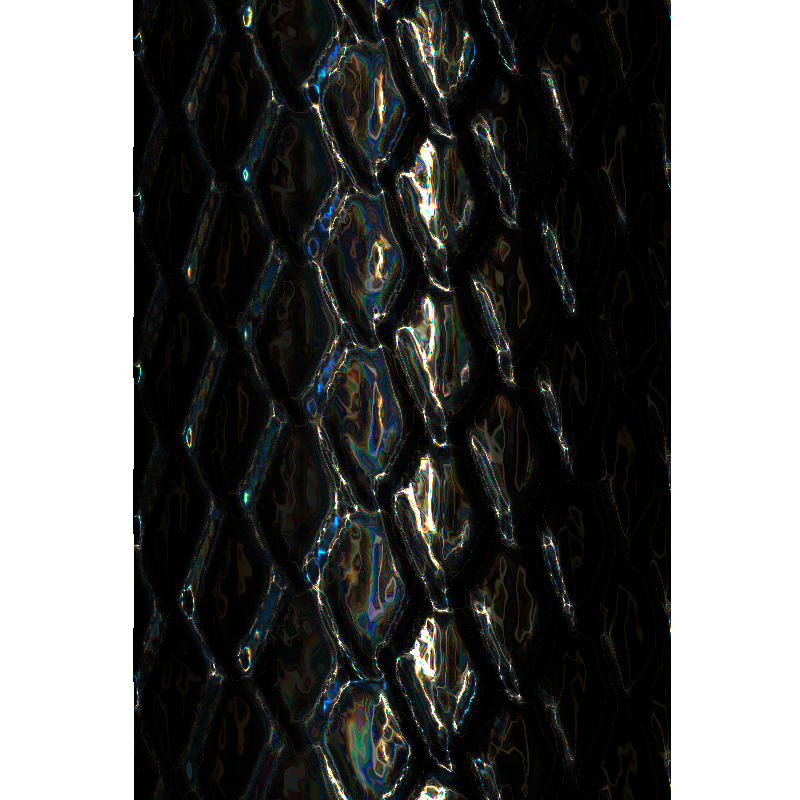
\includegraphics[scale=0.45]{appendix/flss.png}
    \label{fig:appendixcompflsselaphe}
  }
~
  \subfigure[NMM approach]{
    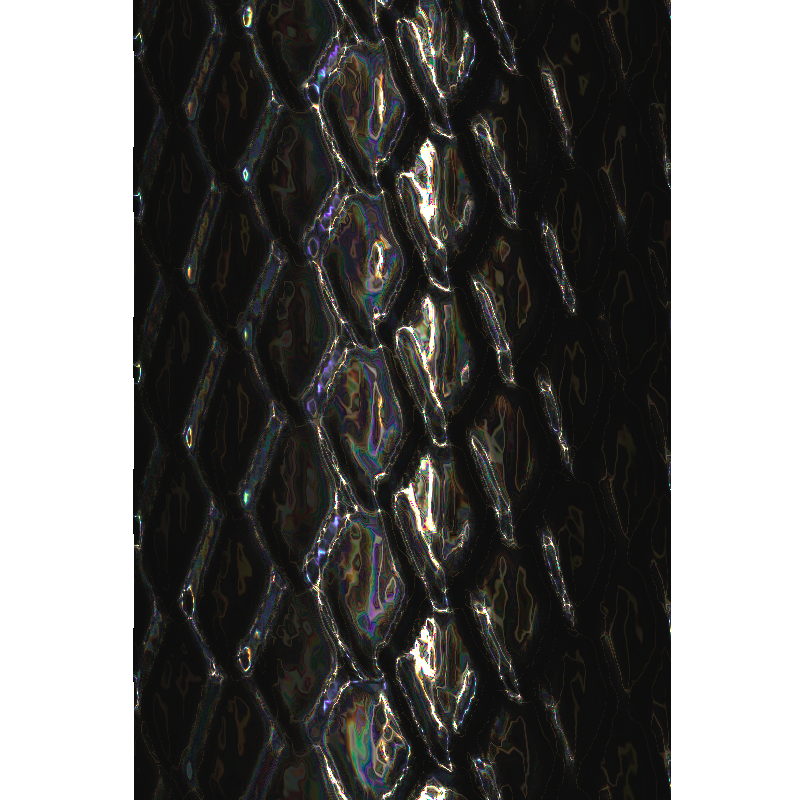
\includegraphics[scale=0.45]{appendix/nmm.png}
    \label{fig:appendixcompnmmlaphe}
  }
~
\caption[Comparing NMM Approach with FLSS Approach]{Comparing the FLSS rendering approach by the NMM approach by rendering an Elaphe grating.}
\label{fig:appendixflssvsnmm}
\end{figure}

In order to address this color-tone issue let us revisit the idea of how we actually compute our color values. For this purpose let us consider the equation $\ref{eq:tristimrad}$ which tells us how to compute CIE XYZ color values. One particular example is the compuation of the lumminance $Y$ which is equal to:

\begin{align}
Y = \int_{\Lambda}L_\lambda(\omega_r)\overline{y}(\lambda)d\lambda \nonumber
\end{align}

In this formulation we integrate over the whole wavelength spectrum $\Lambda$ in oder to compute an anctual color value for $Y$. However, in the NMM approach we perform a \emph{non-uniform} integration over the wavelength spectrum. Instead of directly integrating over the wavelenght spectrum we integrate uniformly over the minimum and maximum wavenumber as explained in section $\ref{sec:nmmapproach}$. Thus, we no longer integrate over the wavelength spectrum we rather integrate over the corresponding wavenumber range $[N_{min}, N_{min}]$. Hence, this depicts a change of integration variables. Unfortunately, I have not taken care of this factor in the NMM approach. In the following I describe what this factor is equal to. \\

The wavenumber for a given wavelength $\lambda$ is equal to

\begin{align}
  k = \frac{2 \pi}{\lambda} \nonumber
\end{align}

For the NMM approach integrate over $dk$ instead over $d\lambda$. By rearranging the definition of the wavnumber $k$ we get the following identitiy for the wavelength:

\begin{align}
  \lambda = \frac{2 \pi}{k} \nonumber
\end{align}

thus, the integrations variable change factor between $d\lambda$ and $dk$ can be computed as the following:

\begin{alignat}{4}
& \frac{d\lambda}{dk} &&= \frac{d}{dk} \left(\frac{2 \pi}{k} \right) = \frac{2 \pi}{k^2}  \nonumber \\
\Rightarrow{} & d\lambda &&= \frac{2 \pi}{k^2} dk \nonumber
\end{alignat}

This will lead us to the final representation for performing an intgration over the wavenumber range:

\begin{align}
Y 
&= \int_{\Lambda}L_\lambda(\omega_r)\overline{y}(\lambda)d\lambda \nonumber \\
&= \int_{N_{min}}^{N_{max}} L_k(\omega_r)\overline{y}(k) \frac{2 \pi}{k^2} dk
\label{eq:wavenumberintegration}
\end{align}
